
\documentclass{article}
\usepackage{hyperref}

\usepackage{graphicx}

\title{Fiberassign performance}
\author{Jaime E. Forero-Romero \footnote{{\texttt{j.e.forero.romero@gmail.com}}}\\Universidad de los Andes}
\date{\today}

\begin{document}
\maketitle
\begin{abstract}
In this document I show that fiberassign meets the desired performance
in terms of fiber usage for science targets, calibration targets,
sky-monitoring locations and Guide/Focus/Alignment targets. 
\end{abstract}

\section{Introduction}
{\texttt fiberassign} is the software that performs the assignment of
fibers to DESI targets. 

The following are the minimal requirements on its performance
\begin{itemize}
\item Fiber assignment uses required fraction of fibers IN.DAT-7002
\item Fiber assignment provides sufficient calibration fibers IN.DAT-7003
\end{itemize}
In this document I present the results of running {\texttt
  fiberassign} on targets from DR7 to demonstrate how the two
requirements mentioned above are met. 
Furthermore I list some computational performance results to
understand how long does it take to run the code and how many
resources does it use.

\section{Software and input data}

For this report I use tag {\texttt 0.10.1} of {\texttt fiberassign}. 

The input targetting data comes from DR7. On NERSC the files can be found here:
{\texttt{/project/projectdirs/desi/target/catalogs/dr7.1/PR372/}}

The targeting files need to be prepared in order to pass them to
fiberassign.
The code that prepares the data and runs fiberassign can be found
here:
\url{https://github.com/forero/fiberassign_explore/blob/master/main.py}.
The script needs to be executed as {\texttt{python main.py --program dark
--size large}} to produce the outputs analized in this report.


\section{Results}


We only use target that can be observed in dark time. 
With this restriction we end up with 7098 DESI tiles that correspond
to dark time and overlap with the DR7.1 footprint. 
This selection returns 36M targets, 1.3M standard stars and
25M sky locations.

Runnig this code on a Cori login node takes 2 hours to run an uses a
peak of 38GB of RAM.
The wallclock time is proportional to the number
of tiles. In this case we have that the code assigns on average one
tile per second. 

Figure \ref{fig:single_tile} show the results from an individual
tile. 
Each panel shows different kinds of targes: 
\begin{itemize}
\item SKY: fibers for sky calibration.
\item STD: fibers on standard starts.
\item SCIENCE: fibers on science targets.
\item GFA: targets on Guide/Focus/Aligment cameras.
\item SKYETC: Sky monitoring fibers for the Exposure Time Calculator.
\end{itemize}

\begin{figure}[!h]
\begin{center}
\begin{center}
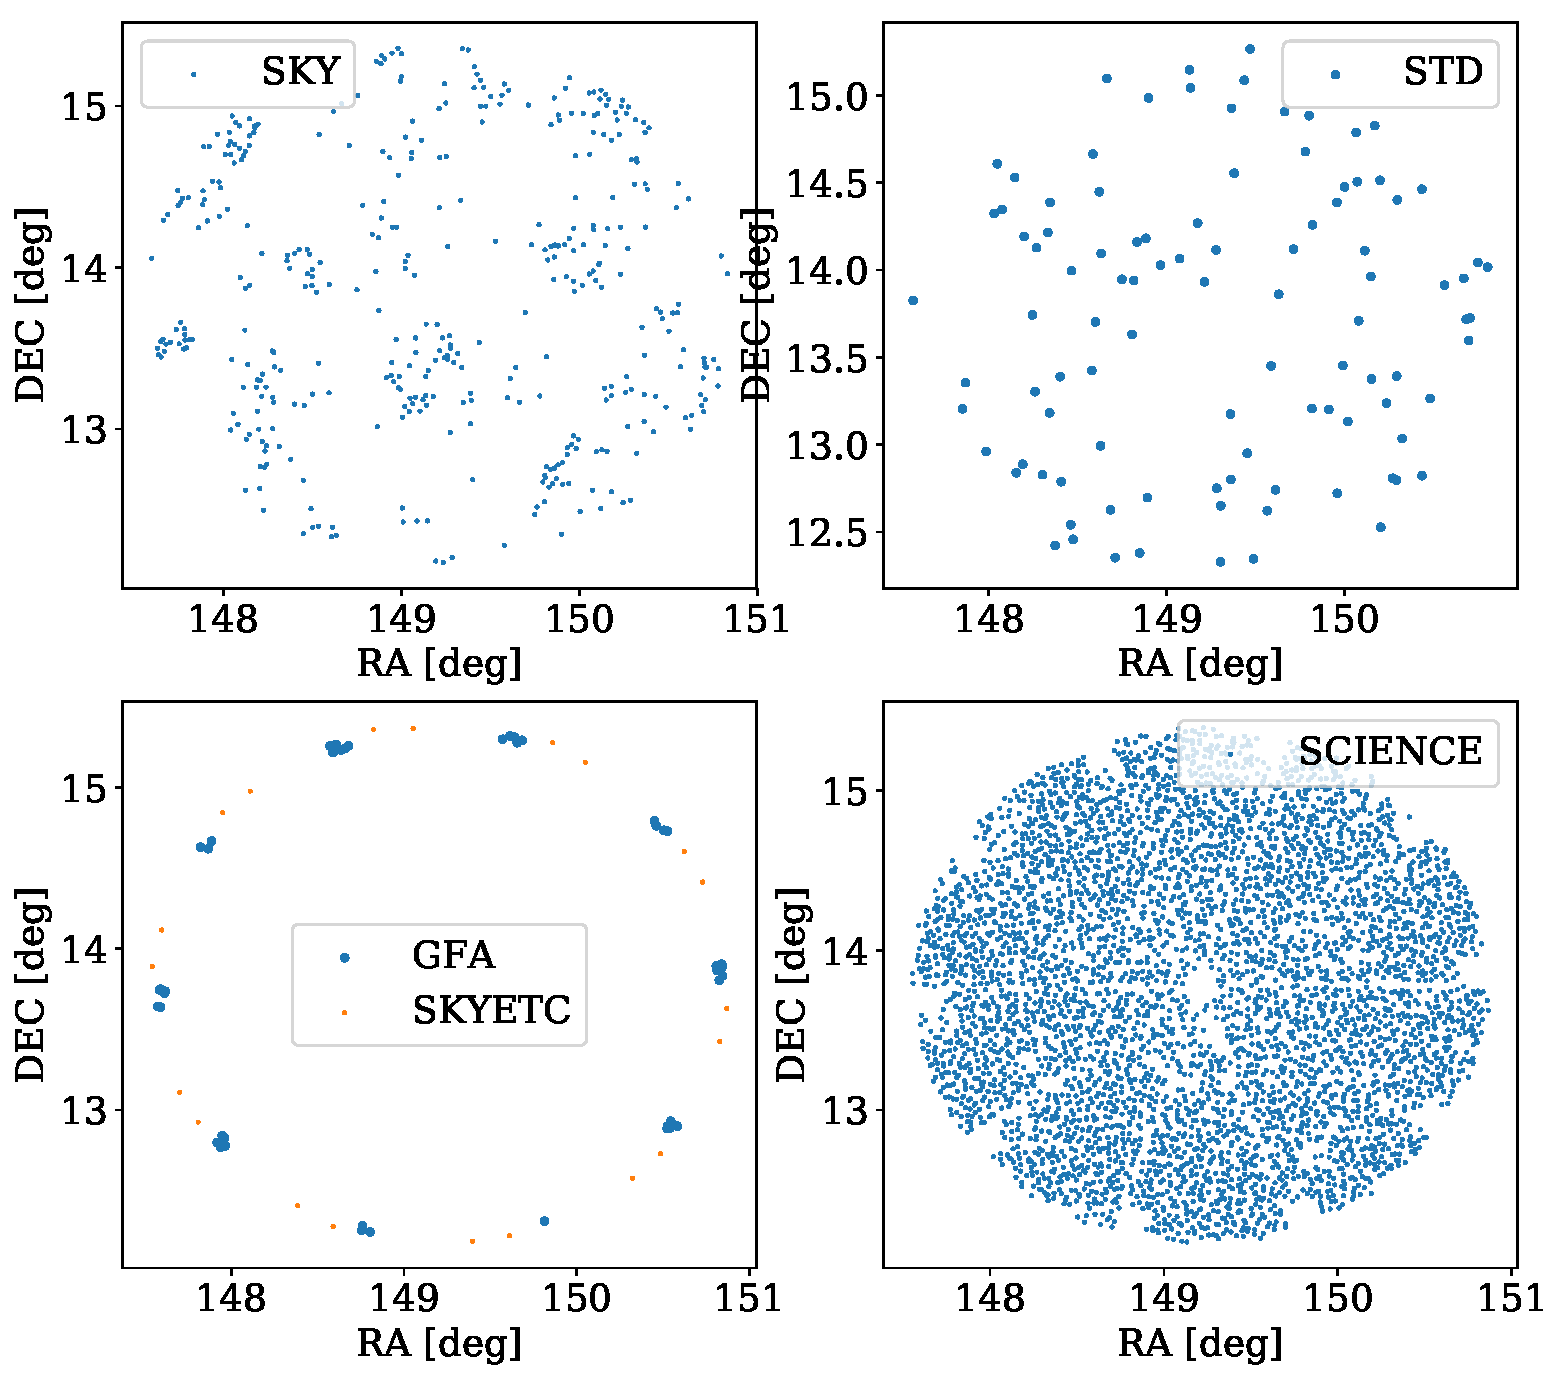
\includegraphics[scale=0.30]{single_tile.pdf}
\end{center}
\caption{Results from a single tile.
Each panel shows the different kinds of targets that are stored
in the outputs.
\label{fig:single_tile}}
\end{center}
\end{figure}

Figure \ref{fig:assigned_ra_dec} show the total number of assigned
fibers for every tile. 
Close to the boundary there are some tiles with a low number of
assigned fibers. 
This is due to the small overlap between those tiles and the DR7.1
footprint; from the beginning a small number of targets are available
for those targets. 
For most of the tiles all the 5K fibers are assigned.

\begin{figure}[!h]
\begin{center}
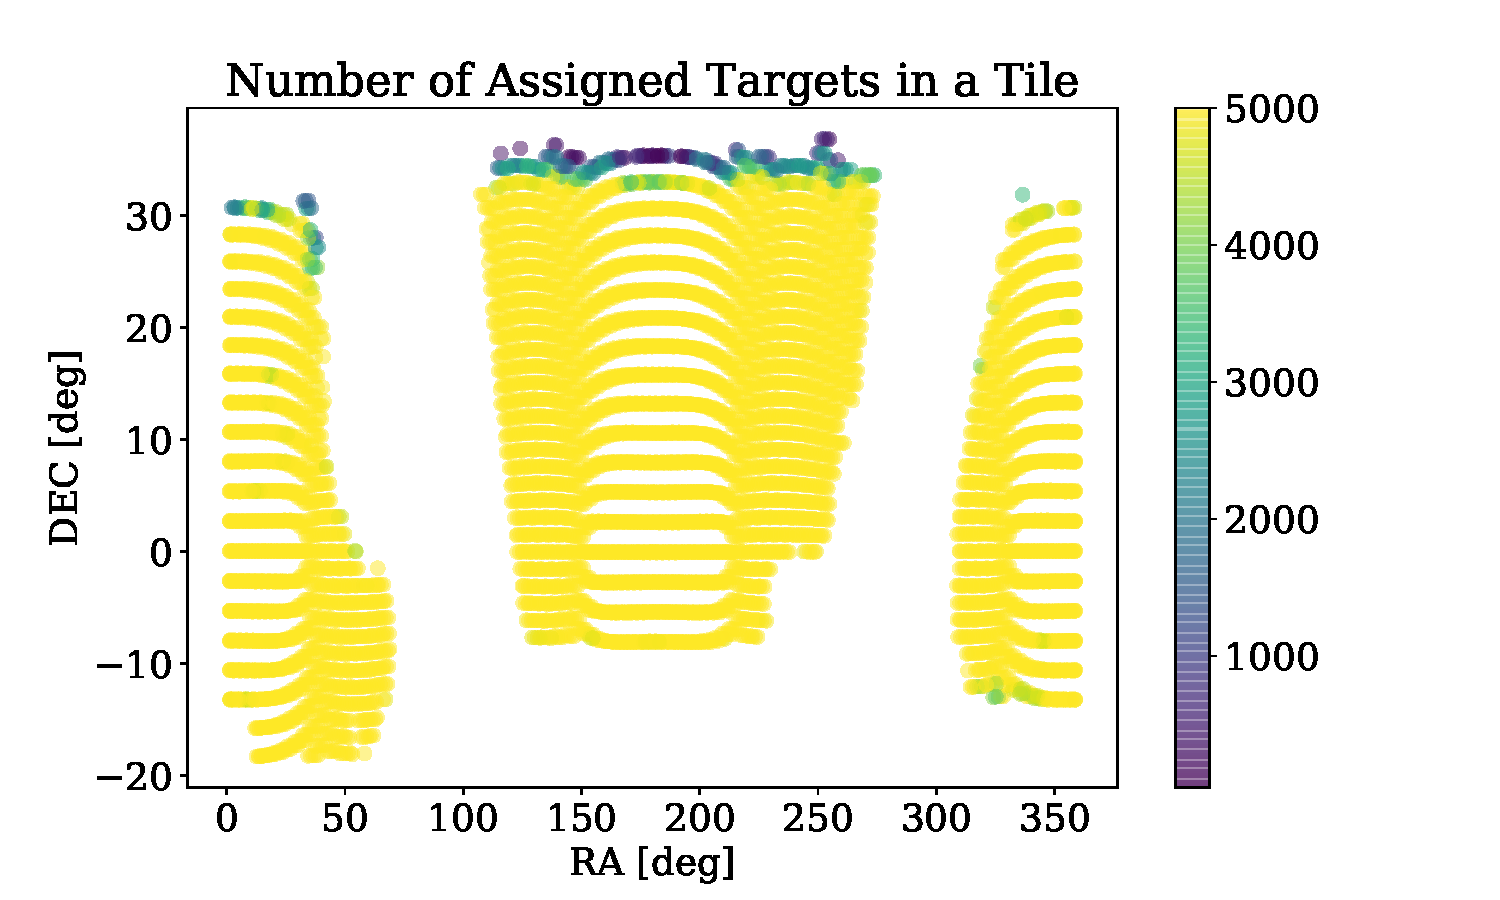
\includegraphics[scale=0.50]{assigned_ra_dec.pdf}
\caption{Total number of assigned fibers for every tile. In the upper
  region the low number of assigned fibers is explained by the small
  overlap with the DR7 footprint.  The same effect is observed for
  some tiles close to the galactic plane.
\label{fig:assigned_ra_dec}}
\end{center}
\end{figure}

In order to produce robust statistics on the number of used fibers for
sky, standards and science targets we discard the tiles above a
declination of $20$ degrees and below $-5$ degrees. 
This cut leave 3884 tiles to be analized.

Figure \ref{fig:used_fibers} shows the histograms of the number of
used fibers per tile.
The label shows the average and the standard deviation computed over
the tiles. 
This Figure shows that on average $99.92\%$ of the fibers are used,
on average $397$ are used for sky locations and $99$ are used for
standard stars. 
On average $4499$ science targets are observed per tile.
The small fluctuations in the number of sky location and standard star fibers
is due to changes in the input number densities for those targets. 
The input sky and stdstar catalogs must be tuned to have everywhere
the desired number of targets per tile. 

Figure \ref{fig:used_fibers} demonstrated that fiber assignement uses
the required fraction of fibers and provides sufficient calibration
targets. 


\begin{figure}[!h]
\begin{center}
\begin{center}
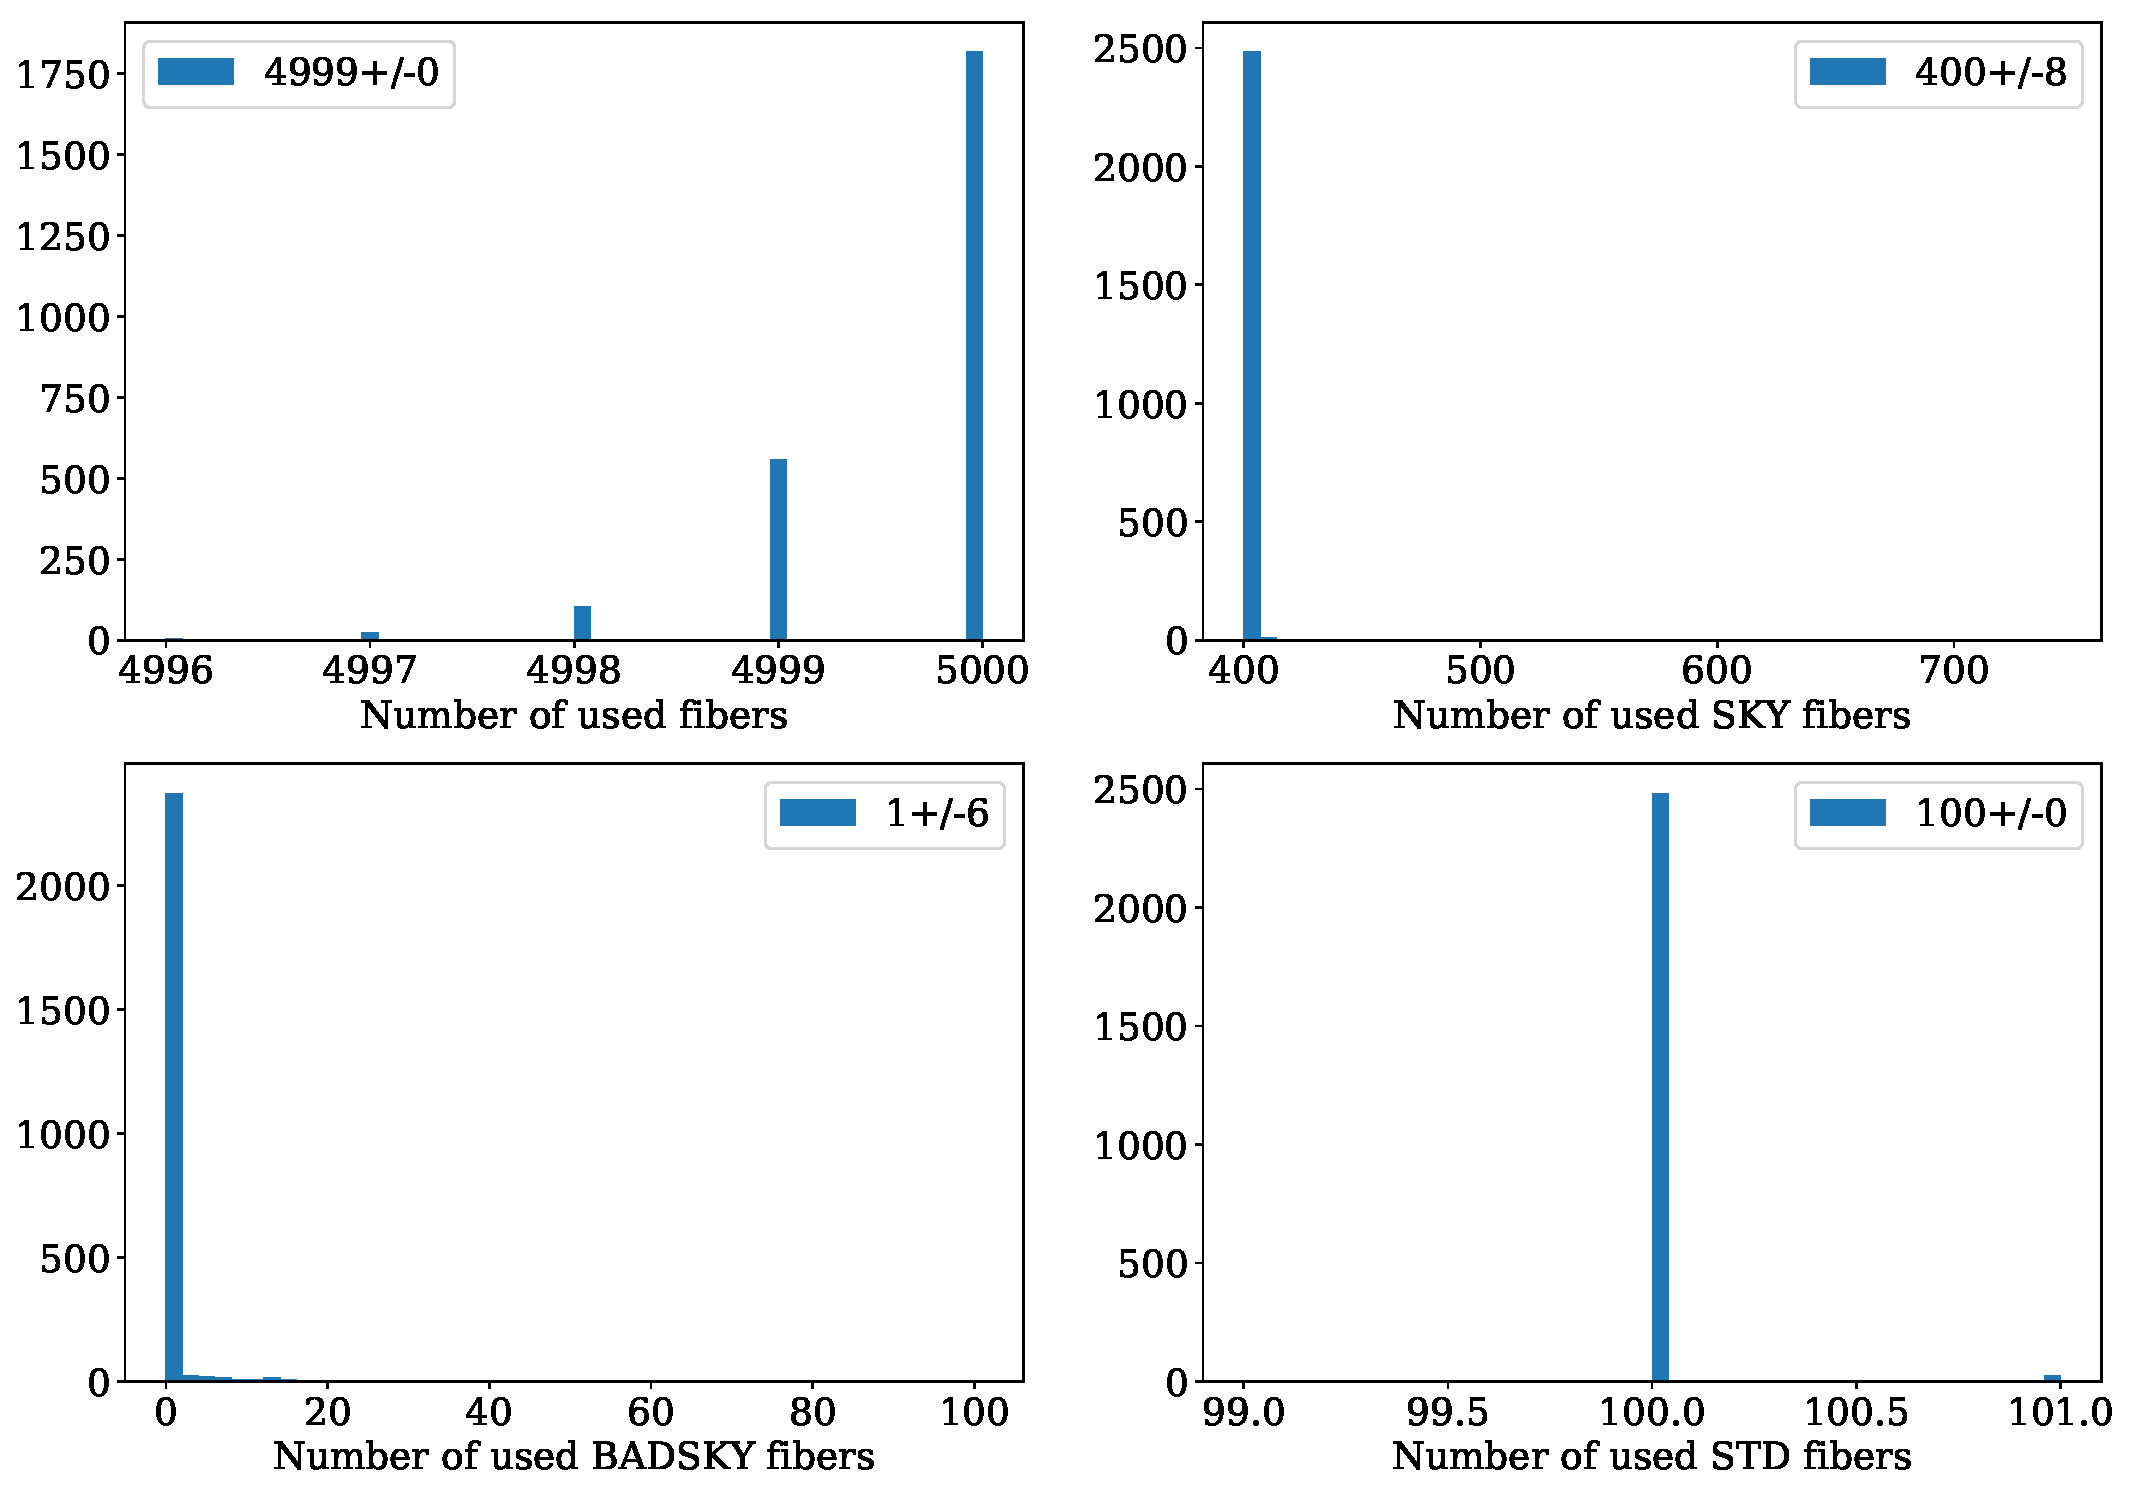
\includegraphics[scale=0.35]{used_fibers.pdf}
\end{center}
\caption{Total number of assigned fibers for every tile. In the upper
  region the low number of assigned fibers is explained by the small
  overlap with the DR7 footprint.  The same effect is observed for
  some tiles close to the galactic plane.
\label{fig:used_fibers}}
\end{center}
\end{figure}

\end{document}
